%%% Local Variables:
%%% mode: latex
%%% TeX-master: ../main.tex
%%% End:

\chapter{用法示例}
\echapter{Example}
\label{cha:example}

\section{插图}
\esection{Figure}

\begin{figure}[!htbp]
  \centering
  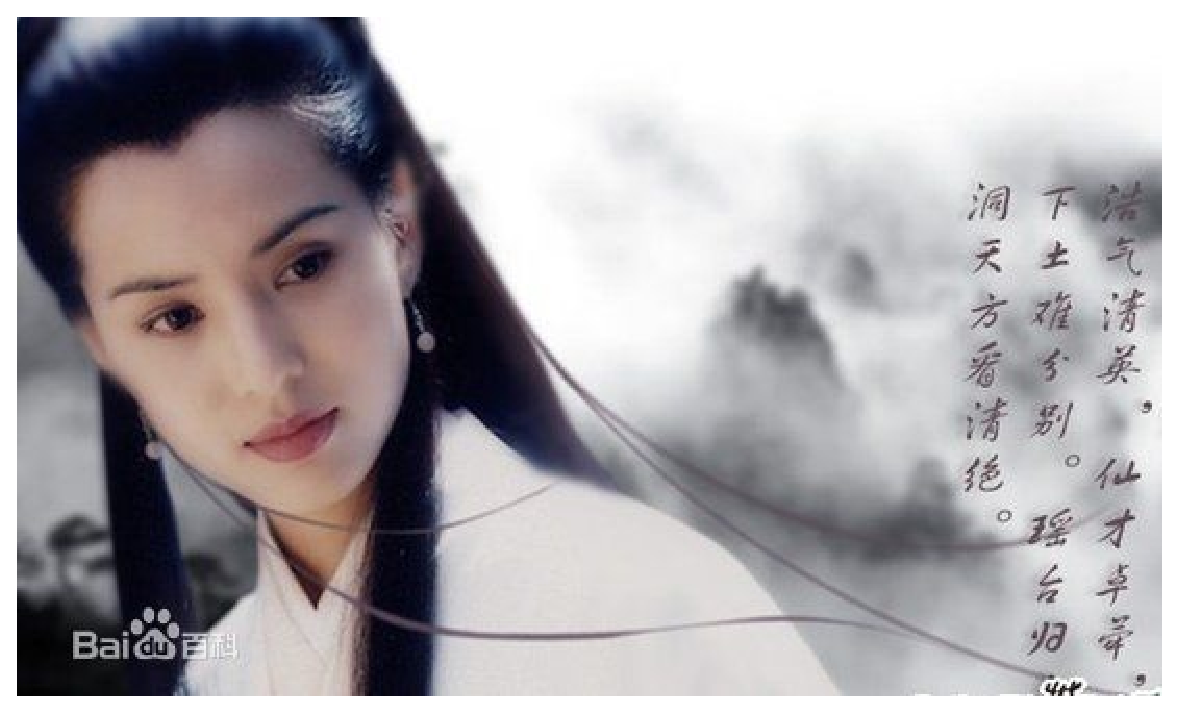
\includegraphics[width=\textwidth]{lrt}
  \caption{香中别有韵,清极不知寒}
  \label{fig:lrt}    
\end{figure}

图\ref{fig:lrt}是一个插图的例子。

图\ref{fig:lrt2}是另一个插图的例子。

\begin{figure}[!htbp]
  \centering
  
\includegraphics[height=3.5in]{lrt2}
  \caption{翩若游龙,宛若惊鸿}
  \label{fig:lrt2}    
\end{figure}


\section{表格}
\esection{Table}

\begin{table}[htbp]
  \centering
  \caption{这是一个自动编号的表格例子}
  \label{tab:tbl}
  \begin{tabular}[c]{|c|m{0.8in}|c|c|c|c|c|}\hline
    \multicolumn{2}{|c|}{Network Topology} & \# of nodes & 
    \multicolumn{3}{c|}{\# of clients} & Server \\\hline
    GT-ITM & Waxman Transit-Stub & 600 &
    \multirow{2}{2em}{2\%}& 
    \multirow{2}{2em}{10\%}& 
    \multirow{2}{2em}{50\%}& 
    \multirow{2}{1.2in}{Max. Connectivity}\\\cline{1-3}
    \multicolumn{2}{|c|}{Inet-2.1} & 6000 & & & &\\\hline
    \multirow{2}{1in}{blabla} & ban  & ban &\multicolumn{4}{c|}{\multirow{2}*{\sduthesis}}\\\cline{2-3}
    & \multicolumn{2}{c|}{ABCDEF} &\multicolumn{4}{c|}{} \\\hline
\end{tabular}  
\end{table}


\section{公式}
\esection{Equation}

首先,有行内公式,如$H~:~\mathcal{C}_n \rightarrow \mathcal{D}_n = \{0,1\}^\lambda$。

然后,有独立成行的不带编号的公式,如
$$
\forall\mathbf{y}\in\Lambda,\quad\mathcal{D}_{\Lambda,s,\mathbf{c}}(\mathbf{y})=\frac{\rho_{s,\mathbf{c}}(\mathbf{y})}{\rho_{s,\mathbf{c}}(\Lambda)}
$$

接下来,就是正常的带编号的公式了,如
\begin{equation}
  \mathbf{Adv}^{eu\mbox{-}acma}_{\Pi}(\mathcal{A}) =  \Pr \left[\mathsf{Sig}\mbox{-}forge_{\mathcal{A},\Pi}(n) = 1 \right] \leq \mathsf{negl}(n).
\end{equation}


\section{算法}
\esection{Algorithm}

\begin{algorithm}
  \caption{算法名称}
\label{alg:alg}
  \algorithmicrequire 输入参数 \\
  \algorithmicensure 输出结果
  \begin{enumerate}
    \item 步骤1
    \item 步骤2
    \item 步骤3
  \end{enumerate}
\end{algorithm}


\section{定义}
\esection{Definition}

\begin{definition}[格]
\label{def:lattice}
给定一组线性无关的向量$\mathbf{B}=\left\{\mathbf{b}_1,\cdots,\mathbf{b}_n\right\}\in\mathbb{R}^{m\times n}$,定义
\begin{equation}
\mathcal{L}(\mathbf{B})=\mathcal{L}(\mathbf{b}_1,\cdots,\mathbf{b}_n)=\left\{\sum_{i\in[n]}x_i\mathbf{b}_i\mid x_i\in\mathbb{Z}\right\}
\end{equation}
为$\mathbf{B}$上的格。其中,线性无关向量组$\mathbf{B}$称作格的\textit{基},$m$和$n$分别称作格的\textit{维}和\textit{秩}。
\end{definition}

定义\ref{def:lattice}是一个定义的例子。


\section{定理}
\esection{Theorem}

\begin{lemma}
\label{lem:basis}
      $\{\mathbf{b}_1,\cdots,\mathbf{b}_n\}$是(有序)基,另一有序基$\{\mathbf{d}_n,\cdots,\mathbf{d}_1\}$是前者对偶基的逆序,那么$\tilde{\mathbf{d}_i}=\tilde{\mathbf{b}_i}/\lVert\tilde{\mathbf{b}_i}\rVert^2(i\in[n])$。
\end{lemma}

引理\ref{lem:basis}是一个引理的例子。其它定理环境参见 sduthesis.pdf 3.6节数学环境。


\section{证明}
\esection{Proof}

\begin{proof}
这是一个证明环境,证明结束的地方会显示一个小黑块。
\end{proof}


\section{其它}
\esection{Others}

不带编号列表:

\begin{itemize}
  \item 无编号
  \item 每项前面有小圆点
  \item 可嵌套
  \begin{itemize}
    \item 最多嵌套3层
    \begin{itemize}
      \item 最多嵌套3层
      \begin{itemize}
        \item 最多嵌套3层
      \end{itemize}
    \end{itemize}
  \end{itemize}
  \item 无编号
\end{itemize}

编号列表:

\begin{enumerate}
  \item 有编号
  \item 可嵌套
  \begin{enumerate}
    \item 第1层嵌套
    \item 最多嵌套3层
    \begin{enumerate}
      \item 最多嵌套3层
        \begin{enumerate}
          \item 最多嵌套3层
        \end{enumerate}
    \end{enumerate}
  \end{enumerate}
  \item 这是顶层条目
\end{enumerate}


%%%
%%% End of File
%%%
